\documentclass[11pt,a4paper]{article}
\usepackage{fontspec}
\usepackage[english]{babel}
\usepackage[margin=2.1cm]{geometry}
\usepackage{booktabs,array,tabularx,longtable,makecell}
\usepackage{xcolor}
\usepackage{amssymb}
\usepackage{graphicx}
\usepackage{pgfplots}
\pgfplotsset{compat=1.17}
\PassOptionsToPackage{hyphens}{url}
\usepackage[hidelinks]{hyperref}
\usepackage{enumitem}
\setlist{nosep,leftmargin=1.4em}
\emergencystretch=3em

\definecolor{impl}{HTML}{3B6EA8}
\definecolor{rev}{HTML}{8FB3DA}

\title{Sweatshop on P-Chess: the learning course\\\large First unit (rook endgames): research, course screens, the Fathom tablebase helper and its cleanups; GPT-6.1 Terra lineup, lane \texttt{learning}}
\author{Foreman, session \texttt{sweatshop/learning/2026-11-07-2234}}
\date{8 November 2026}

\begin{document}
\maketitle

\section*{Your turn}

\textbf{Needs you:}
\begin{enumerate}
  \item \textbf{PR \href{https://github.com/Laginho/P-Chess/pull/44}{\#44} has red CI.} Job
        \texttt{tbprobe-windows} has failed on every push since LEARN-010 merged: the Fathom
        helper built on Windows prints nothing from the accented, spaced folder. The session
        review (below) took it as a finding; see the chat summary for its outcome.
        \texttt{windows-export} also failed on the last two pushes, on a 504 from the Godot download.
  \item \textbf{Confirm or reverse the probe design.} RES-001 (\texttt{Needs your call}) showed that
        Stockfish's UCI never gives each move's distance to zeroing. Its review reserved the change
        of spec L5 for you, but the proxy split LEARN-006 and created LEARN-010, a native helper
        built from Fathom (MIT), with L5 rewritten in \texttt{703fe57}. Everything after it depends on it.
  \item \textbf{Review: human} on LEARN-004 (stage name ``Endgame foundations'', the 36 positions,
        line lengths, difficulty), LEARN-009 (Home's look) and CLEAN-020 (Home details).
  \item Merge PR \#44 when the above are settled.
\end{enumerate}
\textbf{Nothing for you:} 16 tickets at \texttt{Approve} with \texttt{Review: agent}: CORE-007,
CLOCK-003, CI-005, LEARN-001, 002, 003, 005, 006, 007, 008, 010, REV-011, CLEAN-016, 017, 018, 019.

\textbf{Hand tests} (the lane's feature is finished; every ticket is \texttt{done}):
\begin{itemize}
  \item[$\square$] Fresh profile, open Course: the rating dialog has no skip (Escape, click outside);
        1600 chess.com; the map shows the unit as new; Profile shows the same sentence.
  \item[$\square$] Lucena: a correct 3-move line shows $\surd$ on all three, unit page 1/12 and 100\% first try;
        a slow detour stops at that move, and a passing retry counts as solved, not first try.
  \item[$\square$] A losing move in a hold play-out: the end card at once, with that move and a holding move
        (needs a real Maia: this Linux box has no Lc0).
  \item[$\square$] A real game that reached rook and pawn against rook and lost a draw: the marker in Review, its
        link to the unit, ``From your game'' and Continue.
  \item[$\square$] Windows: the tablebase probe from RES-001's procedure, the release unzipped under an accented
        folder, and the app restart with the saved clock choice (LEARN-002).
\end{itemize}

\section*{What changed}

PR \href{https://github.com/Laginho/P-Chess/pull/44}{\#44}, 20 tickets (14 planned, 6 opened during the run).

\textbf{RES-001}: research only. The 40 Syzygy files the unit needs (45.68~MiB), the Stockfish
19 probe, Maia 1500/1900 on 20 sampled positions, and the finding that UCI gives no per-move
distance to zeroing. \path{docs/research/tablebase.md}.
\textbf{CORE-007}: a game keeps the position it started from, and Maia's requests use it, so
play-outs can start mid-game (\path{core/game.gd}, \path{bot/maia_player.gd}).
\textbf{CLOCK-003}: a 5+5 clock and a ``none'' clock that shows blank and never flags
(\path{core/clock.gd}).
\textbf{CI-005}: \path{scripts/fetch-engine.ps1} fetches and checks the 40 tables into
\path{engine/tablebase/}, and the release requires them.
\textbf{LEARN-001}: entering the course asks for your rating once and turns it into the Maia
level; Profile edits it (\path{ui/rating_dialog.gd}, \path{core/course.gd}).
\textbf{LEARN-002}: the course map and the unit page, with progress and a saved clock choice.
Reopened once: a pending review check hid a failed one, so ``needs review'' vanished; the cause
was the status selection in \path{core/course.gd}.
\textbf{LEARN-003}: the theory screen, with the goal, search terms to copy and the path to
Solving (\path{ui/theory.gd}).
\textbf{LEARN-004}: the unit's content, 12 practice and 18 test positions plus 6 play-outs, each
checked against the tablebase (\path{data/course/rook-endgames.json}).
\textbf{LEARN-005}: the Solving board, where you enter a line with legal moves without the pieces
moving. Reopened once: move numbers were wrong when Black starts, and Enter wiped an unfinished
line while Clear had focus, both in \path{ui/solving.gd}.
\textbf{LEARN-010}: a small native helper built from Fathom answers each move's result and distance
to zeroing over the same pipe as the engines (\path{native/tbprobe/main.c},
\path{engine/tablebase.gd}). Reopened twice: the adapter let malformed or out-of-order helper
lines through, during a search and then during start-up, because \path{engine/uci.gd} drops lines
it is not waiting for. \textbf{Risk:} its Windows build fails in CI.
\textbf{LEARN-006}: grading a line against the tablebase and the feedback after it
(\path{core/grader.gd}).
\textbf{LEARN-007}: play-outs against Maia from the course position, each move judged before
Maia replies; they never enter History or stats (\path{ui/playout.gd}).
\textbf{LEARN-008}: the unit's pass test, against a perfect tablebase opponent, with retries and
mastery (\path{ui/pass_test.gd}).
\textbf{LEARN-009}: Home's Continue with its position preview, and the 7- and 30-day review
checks (\path{ui/home.gd}).
\textbf{REV-011}: Review marks a move that threw away a rook-and-pawn-against-rook result and
sends that position to the unit as ``From your game'' (\path{ui/review.gd}).
\textbf{CLEAN-016 to 020}: the rating dialog reuses the shared validator; course saves share one
write sequence; the hold rule text follows its setting; pass-test play-outs share one teardown;
Home's icons, Continue arrow and course summary match the design.

\section*{Record}

\textbf{\$39.53} at API list price over 50 stages, all priced: \texttt{gpt-6.1-terra xhigh}
implementing \$15.55 (21), \texttt{gpt-6.1-sol xhigh} implementing \$6.94 (5) and reviewing
\$17.04 (24). Codex quota: 10 points of the weekly window from a 37\% baseline (22:03), no reset:
Terra 4, Sol 6 (1 implementing, 5 reviewing); three threads outside the stages spent 0. The total
is exact; each stage is $\pm$1 point. The proxy (\texttt{opus-5.5 xhigh}, Claude) is not in these numbers.

\section*{What went wrong}

The Windows side of the new tablebase helper was never run before approval. LEARN-010 was split
out mid-run by the proxy, built and tested on Linux only, and approved with Windows ``pending''.
The windows-latest smoke job it added then failed on every push, and nobody read CI until the run ended.

\begin{enumerate}
  \item Make a red check on the session PR stop the driver, or at least show in its line: the
        job ran 7 times while 9 more tickets merged on top.
  \item When a ticket adds a CI job for a platform the machine lacks, its review should wait for
        that job on a pushed branch, not approve on ``pending''.
  \item Fix the driver's test-file pattern \verb![._-](test|spec)\.[^/.]+$!: it calls
        \path{ui/pass_test.gd} a test and parked a valid LEARN-008 handoff (unparked by hand).
\end{enumerate}

\appendix
\part*{Registro}

\section*{Timeline}

{\small
\begin{tabularx}{\linewidth}{@{}lX@{}}
\toprule
7 Nov 22:37 & Clone made from origin on the Linux box; driver launched (default lineup). Reuses the
        session branch a killed Windows driver had opened (empty commit \texttt{6b92979}). \\
22:38--00:00 & RES-001, CORE-007, CLOCK-003, CI-005, LEARN-001 merged, none reopened. \\
00:01--00:36 & LEARN-002 reopened once (status precedence), merged. \\
00:36--02:06 & LEARN-003, LEARN-004 (review adds a missing assertion), LEARN-005 (reopened once). \\
02:06--02:21 & LEARN-006 on the hard model asks; proxy splits off LEARN-010; no code. \\
02:21--02:43 & CLEAN-016, CLEAN-017 merged. \\
02:43--03:26 & LEARN-010 reopened twice; driver parks it and ends (PR \#44, 11 tickets). \\
03:28 & Foreman's reopen diagnosis and consolidated review committed; driver relaunched. \\
03:29--04:17 & LEARN-010 merged on round 3; LEARN-006 merged. \\
04:17--05:34 & LEARN-007 merged; LEARN-008 parked by the test-file false positive; CLEAN-018 merged;
        driver ends. \\
05:35 & LEARN-008 restored to \texttt{to-review}; driver relaunched. \\
05:35--07:24 & LEARN-008, LEARN-009 merged; REV-011 asks, proxy answers, merged; CLEAN-019,
        CLEAN-020 merged. Nothing left in the lane. \\
\bottomrule
\end{tabularx}
}

\section*{Per stage}

{\scriptsize
\setlength\tabcolsep{3pt}
\begin{longtable}{@{}llllrrrrrl@{}}
\toprule
When & Ticket & Stage & Model & Min & In & Cache & Out & Cost & Outcome \\
\midrule
\endhead
22:53 & RES-001 & impl & terra xhigh & 16 & 10.7M & 99\% & 27k & 0.792 & to-review \\
22:58 & RES-001 & review & sol xhigh & 5 & 2.5M & 95\% & 14k & 0.637 & merged \\
23:06 & CORE-007 & impl & terra xhigh & 8 & 3.9M & 98\% & 8k & 0.299 & to-review \\
23:09 & CORE-007 & review & sol xhigh & 3 & 1.3M & 94\% & 8k & 0.374 & merged \\
23:20 & CLOCK-003 & impl & terra xhigh & 10 & 4.7M & 98\% & 11k & 0.384 & to-review \\
23:23 & CLOCK-003 & review & sol xhigh & 3 & 1.5M & 93\% & 9k & 0.437 & merged \\
23:35 & CI-005 & impl & terra xhigh & 12 & 6.1M & 99\% & 17k & 0.462 & to-review \\
23:40 & CI-005 & review & sol xhigh & 5 & 2.4M & 95\% & 17k & 0.657 & merged \\
23:54 & LEARN-001 & impl & terra xhigh & 14 & 10.6M & 99\% & 25k & 0.762 & to-review \\
00:00 & LEARN-001 & review & sol xhigh & 7 & 4.2M & 95\% & 21k & 1.016 & merged \\
00:20 & LEARN-002 & impl & terra xhigh & 19 & 14.0M & 99\% & 35k & 0.993 & to-review \\
00:25 & LEARN-002 & review & sol xhigh & 5 & 3.3M & 95\% & 16k & 0.772 & reopened \\
00:33 & LEARN-002 & impl & terra xhigh & 8 & 5.5M & 99\% & 8k & 0.386 & to-review \\
00:36 & LEARN-002 & review & sol xhigh & 3 & 1.6M & 94\% & 10k & 0.447 & merged \\
00:54 & LEARN-003 & impl & terra xhigh & 18 & 12.2M & 99\% & 23k & 0.826 & to-review \\
00:58 & LEARN-003 & review & sol xhigh & 4 & 1.9M & 94\% & 11k & 0.525 & merged \\
01:16 & LEARN-004 & impl & terra xhigh & 18 & 11.6M & 99\% & 29k & 0.834 & to-review \\
01:26 & LEARN-004 & review & sol xhigh & 10 & 4.7M & 95\% & 23k & 1.118 & merged \\
01:46 & LEARN-005 & impl & terra xhigh & 20 & 18.1M & 99\% & 33k & 1.192 & to-review \\
01:50 & LEARN-005 & review & sol xhigh & 5 & 2.8M & 94\% & 15k & 0.738 & reopened \\
02:03 & LEARN-005 & impl & terra xhigh & 12 & 7.5M & 99\% & 13k & 0.518 & to-review \\
02:06 & LEARN-005 & review & sol xhigh & 3 & 1.9M & 95\% & 10k & 0.491 & merged \\
02:21 & LEARN-006 & impl & sol xhigh & 15 & 3.5M & 97\% & 17k & 0.685 & split, no code \\
02:28 & CLEAN-016 & impl & terra xhigh & 8 & 1.9M & 98\% & 5k & 0.156 & to-review \\
02:31 & CLEAN-016 & review & sol xhigh & 3 & 1.1M & 94\% & 8k & 0.302 & merged \\
02:40 & CLEAN-017 & impl & terra xhigh & 9 & 4.7M & 99\% & 10k & 0.341 & to-review \\
02:43 & CLEAN-017 & review & sol xhigh & 3 & 1.3M & 93\% & 8k & 0.379 & merged \\
03:05 & LEARN-010 & impl & sol xhigh & 22 & 8.5M & 98\% & 56k & 1.739 & to-review \\
03:09 & LEARN-010 & review & sol xhigh & 4 & 2.7M & 95\% & 14k & 0.672 & reopened \\
03:21 & LEARN-010 & impl & sol xhigh & 12 & 4.7M & 98\% & 20k & 0.897 & to-review \\
03:26 & LEARN-010 & review & sol xhigh & 5 & 3.7M & 94\% & 19k & 0.983 & reopened \\
03:46 & LEARN-010 & impl & sol xhigh & 17 & 6.6M & 98\% & 34k & 1.316 & to-review \\
03:50 & LEARN-010 & review & sol xhigh & 4 & 3.1M & 95\% & 13k & 0.732 & merged \\
04:13 & LEARN-006 & impl & sol xhigh & 23 & 12.8M & 98\% & 59k & 2.301 & to-review \\
04:17 & LEARN-006 & review & sol xhigh & 4 & 3.1M & 93\% & 14k & 0.835 & merged \\
04:42 & LEARN-007 & impl & terra xhigh & 25 & 26.7M & 99\% & 47k & 1.747 & to-review \\
04:58 & LEARN-007 & review & sol xhigh & 16 & 7.9M & 97\% & 31k & 1.510 & merged \\
05:20 & LEARN-008 & impl & terra xhigh & 22 & 22.1M & 99\% & 40k & 1.471 & parked (false positive) \\
05:30 & CLEAN-018 & impl & terra xhigh & 10 & 3.2M & 98\% & 9k & 0.259 & to-review \\
05:34 & CLEAN-018 & review & sol xhigh & 3 & 1.3M & 94\% & 9k & 0.381 & merged \\
05:47 & LEARN-008 & review & sol xhigh & 11 & 8.5M & 98\% & 22k & 1.454 & merged \\
06:19 & LEARN-009 & impl & terra xhigh & 32 & 32.6M & 99\% & 55k & 2.234 & to-review \\
06:25 & LEARN-009 & review & sol xhigh & 6 & 3.4M & 95\% & 16k & 0.843 & merged \\
06:28 & REV-011 & impl & terra xhigh & 3 & 1.2M & 95\% & 5k & 0.141 & asked, blocked \\
06:43 & REV-011 & impl & terra xhigh & 14 & 8.5M & 99\% & 24k & 0.648 & to-review \\
06:47 & REV-011 & review & sol xhigh & 4 & 2.4M & 94\% & 13k & 0.627 & merged \\
07:00 & CLEAN-019 & impl & terra xhigh & 12 & 4.4M & 98\% & 12k & 0.345 & to-review \\
07:03 & CLEAN-019 & review & sol xhigh & 3 & 1.5M & 92\% & 8k & 0.446 & merged \\
07:17 & CLEAN-020 & impl & terra xhigh & 14 & 10.6M & 99\% & 25k & 0.757 & to-review \\
07:24 & CLEAN-020 & review & sol xhigh & 6 & 2.4M & 95\% & 17k & 0.665 & merged \\
\midrule
 & & & & 518 & 327.4M & & & 39.53 & \\
\bottomrule
\end{longtable}
}

\begin{center}
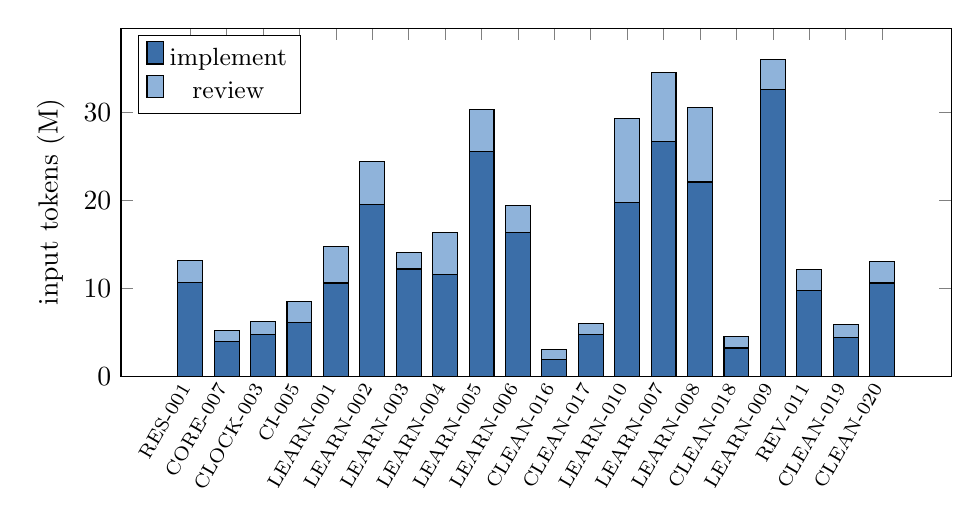
\begin{tikzpicture}
\begin{axis}[ybar stacked, bar width=9pt, width=\linewidth, height=6cm,
  symbolic x coords={RES-001,CORE-007,CLOCK-003,CI-005,LEARN-001,LEARN-002,LEARN-003,LEARN-004,LEARN-005,LEARN-006,CLEAN-016,CLEAN-017,LEARN-010,LEARN-007,LEARN-008,CLEAN-018,LEARN-009,REV-011,CLEAN-019,CLEAN-020},
  xtick=data, x tick label style={rotate=60,anchor=east,font=\scriptsize}, ylabel={input tokens (M)}, ymin=0,
  legend style={at={(0.02,0.98)},anchor=north west,font=\small}]
\addplot[fill=impl] coordinates {(RES-001,10.7) (CORE-007,3.9) (CLOCK-003,4.7) (CI-005,6.1) (LEARN-001,10.6) (LEARN-002,19.5) (LEARN-003,12.2) (LEARN-004,11.6) (LEARN-005,25.6) (LEARN-006,16.3) (CLEAN-016,1.9) (CLEAN-017,4.7) (LEARN-010,19.8) (LEARN-007,26.7) (LEARN-008,22.1) (CLEAN-018,3.2) (LEARN-009,32.6) (REV-011,9.7) (CLEAN-019,4.4) (CLEAN-020,10.6)};
\addplot[fill=rev] coordinates {(RES-001,2.5) (CORE-007,1.3) (CLOCK-003,1.5) (CI-005,2.4) (LEARN-001,4.2) (LEARN-002,4.9) (LEARN-003,1.9) (LEARN-004,4.7) (LEARN-005,4.7) (LEARN-006,3.1) (CLEAN-016,1.1) (CLEAN-017,1.3) (LEARN-010,9.5) (LEARN-007,7.9) (LEARN-008,8.5) (CLEAN-018,1.3) (LEARN-009,3.4) (REV-011,2.4) (CLEAN-019,1.5) (CLEAN-020,2.4)};
\legend{implement, review}
\end{axis}
\end{tikzpicture}
\end{center}

Wasted: the four reopened reviews and the stage 2 runs that answered them, \$6.48 (LEARN-002
\$1.16, LEARN-005 \$1.26, LEARN-010 \$4.07 across two rounds and three re-implementations,
counting the extra review). LEARN-006's first attempt (\$0.69) wrote no code but produced the
split; REV-011's first attempt (\$0.14) only asked. LEARN-008's park cost nothing: its work was kept
and reviewed as handed off. The heaviest tickets by input were LEARN-009 (36.0M), LEARN-007 (34.6M)
and LEARN-008 (30.6M): screens that reach Main, Home and the course module at once.

\section*{Comparison with previous runs}

From \texttt{run-log.md}. \texttt{audit-fixes} (6 Nov, Windows): \$6.07 for 6 (\$1.01 each), no reopens.
\texttt{review-explore} (5 Nov): \$11.40 for 3 (\$3.80 each), four reopens. This run: \$39.53 for 20
(\$1.98 each), 4 of 24 reviews reopened (17\%). It is the longest P-Chess run so far (8\,h47, three
launches), and a feature lane, so it compares with \texttt{review-explore} rather than with the bounded
fixes of \texttt{audit-fixes}.

\section*{Observations per model}

\begin{itemize}
  \item \textbf{gpt-6.1-terra xhigh, stage 2} (21 stages, 3--32~min): 15 tickets on its first
        attempt. Two reopens (LEARN-002, LEARN-005), both explicit criteria it missed. It took care
        of test-first strictly (LEARN-008: 14 commits, each pure). It asked well on REV-011: a
        real gap in the data, not a guess.
  \item \textbf{gpt-6.1-sol xhigh, stage 2 (hard)} (5 stages): LEARN-006 stopped before writing
        code and took the contract question to the proxy, which is what the ticket-flow asks.
        LEARN-010 needed three rounds: its first repair claimed start-up coverage without a test for it.
  \item \textbf{gpt-6.1-sol xhigh, review} (24 stages, 3--16~min): reopens were reproduced, with
        exact repair instructions. Two misses: LEARN-010's round 1 read malformed output only
        during a search (round 2 found the start-up path, already present), and LEARN-010 was
        approved with its own new Windows CI job never run. It filed five \texttt{CLEAN-*} tickets
        instead of widening scope, and the driver ran all five.
  \item \textbf{opus-5.5 xhigh, proxy}: six decisions (below). One call's answer started with a
        preamble line, and \path{proxy.ps1} rejected it, so REV-011's stage reported a proxy
        failure. The driver's second call gave the same value (3 moves) but put it in the data
        file instead of a code constant.
\end{itemize}

\section*{Driver and runtime issues}

\begin{enumerate}
  \item The test-file pattern in \path{driver.ps1} (\verb![._-](test|spec)\.[^/.]+$!) matched the
        production screen \path{ui/pass_test.gd}. LEARN-008 was parked as ``incomplete handoff''. The
        foreman checked the 14 commits and restored \texttt{to-review} (\texttt{9fa4730}).
  \item LEARN-006's planned stop after the proxy's split was logged as \texttt{failed (exit 0), will
        retry} and spent attempt 1.
  \item \path{proxy.ps1} needs \texttt{Decision:} on the first line; an answer with a preamble
        line counts as a failure even with a decision below it.
  \item The main checkout's \path{.git/info/exclude} lacked the run-log, \texttt{*.uid} and
        \texttt{*.import} lines the Windows checkout has; the foreman added them to the new clone.
        After CI-005 and LEARN-010, the ignored \path{engine/tablebase} (a link to the hard disk) and
        \path{engine/tbprobe/} showed as untracked on \texttt{main}, whose \path{.gitignore} lacks them, and
        would have failed Preflight; added to the clone's exclude.
  \item No Linux Lc0 and no display in the clone: six live Maia tests and the headless pixel checks were
        skipped in every gate; Xvfb was used for the clipboard and board captures.
  \item No crash, timeout or API error. Shutdown 0.5--1.8~s per stage.
\end{enumerate}

\section*{Restarts and cleanups}

No crash restart. Two relaunches after foreman fixes: at 03:28, after the LEARN-010 reopen
diagnosis (\texttt{c087ae0}), and at 05:35, after the LEARN-008 restore (\texttt{9fa4730}).
The diagnosis classified the second reopen as an earlier review miss plus an incomplete repair, not
a contract gap. Its consolidated review added three items: phase-aware validation, the exact
\texttt{id name} line, and a non-draw with distance 0. Round 3 merged with no findings.

\section*{Noticed and left alone}

\begin{itemize}
  \item The proxy, not Bruno, approved the change to spec L5 (see Your turn).
  \item CLEAN-017's write and rename failure paths were checked by reading, with no injected
        failure (the ticket asked for no new tests).
  \item Several tickets wrote evidence to \path{/run/media/lage/New Volume/Scratch/}, which is local to
        this machine; the tickets carry the commands.
\end{itemize}

\section*{Human debt and proxy decisions}

No \texttt{Débito humano:} lines in this run's tickets. All six decisions were made by
\texttt{opus-5.5 xhigh}; Codex sessions reached the proxy directly, and one (REV-011) was asked by
the driver after the stage's own call failed to parse.
\begin{itemize}
  \item RES-001 (22:39): \texttt{Proxy decided (opus-5.5 xhigh): proceed on Linux and do not wait for
        a Windows run.} Criterion 2 measured with the Linux build of Stockfish 19; Windows syntax
        pending Bruno; lc0 built natively for criterion 5.
  \item LEARN-002 (00:07): \texttt{Proxy decided (opus-5.5 xhigh): Keep all four parts on the unit page
        and the course-map card; reword criterion 5 so it bans placeholder units and stages, not the
        four fixed parts.}
  \item LEARN-003 (00:43): \texttt{Proxy decided (opus-5.5 xhigh): LEARN-003 adds no book or chapter
        entries.} LEARN-004 supplies them.
  \item LEARN-004 (00:59): \texttt{Proxy decided (opus-5.5 xhigh): Name the stage ``Endgame
        foundations'' and go ahead with the draft content.}
  \item LEARN-006 (02:17): \texttt{Proxy decided (opus-5.5 xhigh): split (B).} The native probe
        becomes LEARN-010; LEARN-006 waits for it.
  \item REV-011 (06:28, asked by the driver): \texttt{Proxy decided (opus-5.5 xhigh)}: add \path{"default_line_length": 3} to the unit file
        and use it for every ``From your game'' position.
\end{itemize}
Receipts: \path{/tmp/sweatshop-proxy/} on this machine, named in each ticket.

\section*{Acceptance}

Spec scenarios, on the integrated session (\texttt{66abb54}, gate 677 passed, 0 failed; real
tablebase tests ran): scenario 4 (review check at 7 days) passed in
\path{test_continue_offers_review_checks_at_seven_and_thirty_days} and two screen tests.
Scenarios 1, 2, 3 and 5 are Bruno's hand checks (Your turn); their automated parts pass. Not
examined: anything on Windows, a real Maia reply, and a person at the screen. Recorded in
\path{.scratch/learning/spec.md} and PR \#44.

\section*{Reopen attribution}

Labelled by the foreman (opus-5.5); every round's reviewer was \texttt{gpt-6.1-sol xhigh}, so
none is self-judged. Rows appended to \path{.scratch/reopen-attribution.md}.

{\small\noindent
\begin{tabularx}{\linewidth}{@{}>{\raggedright\arraybackslash}p{1.9cm}X>{\raggedright\arraybackslash}p{2.7cm}X@{}}
\toprule
Ticket (round) & Finding & Label & Why \\
\midrule
LEARN-002 (1) & a pending review check hides a failed one; ``needs review'' vanishes & S2-explícito/código & criterion 2; no test had the case \\
LEARN-005 (1) & move numbers wrong when Black starts & S2-explícito/código & criterion 5 \\
LEARN-005 (1) & Enter wipes an unfinished line while Clear has focus & S2-explícito/código & criterion 7 \\
LEARN-010 (1) & malformed \texttt{bestmove} tokens and unknown lines during a search succeed & S2-explícito/código & criterion 4 \\
LEARN-010 (2) & invalid lines before the handshake barriers or while idle are dropped & S2-explícito/código & criterion 4; present since the first handoff: review miss (drip-feed) \\
LEARN-004 (0) & the shape test did not require both goals in each pool & S2-explícito/teste & added by the review (\texttt{fdf31ff}) \\
LEARN-010 (--) & Windows smoke probe fails in CI & unclassified & post-approval, \texttt{session-review} \\
\bottomrule
\end{tabularx}
}

Totals: S2-explícito/código 5, S2-explícito/teste 1 (fixed in review), unclassified 1
(post-approval). No S1 or S3. Review miss: LEARN-010 round 2. No review-induced churn.

\section*{Scoreboard}

\texttt{scoreboard.ps1} over this machine's main checkouts (ClassyCall, EasyMath, P-Chess, PhysiSyst,
SIGAA-ME, SynchroNice, slip), with P-Chess read from the lane clone, whose log is identical to the main
checkout's after the copy-back and which alone holds this run's attribution and interventions. Moved since the
\texttt{review-explore} report (the last one from this machine; \texttt{audit-fixes} ran on Windows):
pair \texttt{gpt-6.1-terra xhigh} $\rightarrow$ \texttt{gpt-6.1-sol xhigh} 101 $\to$ 154 reviews, 29\%
$\to$ 24\% reopened (S2 $\geq$23\%); pair \texttt{gpt-6.1-sol xhigh} $\rightarrow$ \texttt{gpt-6.1-sol xhigh}
22 $\to$ 33 reviews, 23\% $\to$ 27\% (LEARN-010's two reopens); proxy-decision (opus-5.5 xhigh) 47 $\to$ 64;
automatic-recovery 130 $\to$ 133.

{\footnotesize
\setlength\tabcolsep{4pt}
\begin{longtable}{@{}lrrrrrr@{}}
\toprule
\textbf{Implementer} & \textbf{\makecell[b]{Stage\\runs}} & \textbf{To review} & \textbf{Failed} & \textbf{Asked} & \textbf{\makecell[b]{Median\\min to\\review}} & \textbf{Cost} \\
\midrule
\endhead
gpt-6-astra medium & 57 & 47 & 1 & 9 & 10m & \$162.72 (57/57 priced) \\
gpt-6.1-sol-fast high & 18 & 16 & 0 & 2 & 10m & \$21.98 (15/18 priced) \\
gpt-6.1-sol-fast max & 14 & 12 & 0 & 2 & 12m & \$31.19 (14/14 priced) \\
opus-5.5 & 42 & 35 & 4 & 3 & 8m & \$15.84 (8/42 priced) \\
gpt-6-luna max & 89 & 61 & 10 & 18 & 17m & \$4.91 (85/89 priced) \\
sonnet-5.5 high & 18 & 17 & 1 & 0 & 7m & \$31.92 (18/18 priced) \\
gpt-6.1-sol high & 311 & 275 & 12 & 24 & 23m & \$839.52 (309/311 priced) \\
gpt-6-astra high & 1 & 0 & 0 & 1 & - & \$3.92 (1/1 priced) \\
opus-5.5 xhigh & 24 & 16 & 8 & 0 & 14m & \$100.17 (22/24 priced) \\
gpt-6.1-sol max & 41 & 29 & 9 & 3 & 24m & \$84.42 (33/41 priced) \\
haiku-5.5 high & 26 & 6 & 15 & 5 & 21m & \$72.08 (24/26 priced) \\
haiku-5.5 xhigh & 4 & 0 & 3 & 1 & - & \$12.29 (4/4 priced) \\
opus-5.5 high & 37 & 21 & 15 & 1 & 12m & \$73.54 (29/37 priced) \\
gpt-6.1-sol xhigh & 44 & 33 & 1 & 0 & 19m & \$99.35 (44/44 priced) \\
gpt-6.1-terra high & 59 & 30 & 27 & 2 & 9m & \$9.45 (34/59 priced) \\
gpt-6.1-terra xhigh & 185 & 155 & 19 & 11 & 15m & \$139.31 (185/185 priced) \\
sonnet & 121 & 75 & 31 & 15 & 7m & \$10.53 (4/121 priced) \\
sonnet-5.5 xhigh & 9 & 8 & 1 & 0 & 25m & \$35.54 (9/9 priced) \\
fable & 5 & 5 & 0 & 0 & 3m & ? \\
gpt-6-luna & 23 & 11 & 10 & 2 & 26m & ? \\
gpt-6-sol & 6 & 5 & 1 & 0 & 17m & ? \\
gpt-5.6-sol & 5 & 4 & 1 & 0 & 17m & ? \\
gpt-6-astra & 18 & 11 & 6 & 1 & 8m & ? \\
sonnet-5 xhigh & 11 & 6 & 2 & 3 & 8m & \$18.09 (11/11 priced) \\
gpt-6-astra low & 2 & 2 & 0 & 0 & 30m & \$19.03 (2/2 priced) \\
\bottomrule
\end{longtable}
\setlength\tabcolsep{2pt}
\begin{longtable}{@{}llrrrrrrr@{}}
\toprule
\textbf{Implementer} & \textbf{Reviewer} & \textbf{Reviews} & \textbf{Reopened} & \textbf{\makecell[b]{Reopen\\rate}} & \textbf{\makecell[b]{Reopened\\for S2}} & \textbf{S2 rate} & \textbf{\makecell[b]{Unclas-\\sified}} & \textbf{\makecell[b]{Fixed in\\review\\for S2}} \\
\midrule
\endhead
gpt-6-astra medium & gpt-6.1-sol max & 37 & 7 & 19\% & 6 & 16\% & 0 & 1 \\
gpt-6.1-sol-fast high & gpt-6.1-sol-fast max & 16 & 2 & 12\% & 2 & 12\% & 0 & 0 \\
gpt-6.1-sol-fast max & gpt-6.1-sol-fast max & 12 & 6 & 50\% & 5 & 42\% & 0 & 0 \\
opus-5.5 & opus-5.5 & 4 & 0 & 0\% & 0 & 0\% & 0 & 0 \\
gpt-6-luna max & opus-5.5 high & 18 & 1 & 6\% & 1 & 6\% & 0 & 0 \\
gpt-6-luna max & gpt-6-sol max & 43 & 23 & 53\% & 22 & 51\% & 0 & 0 \\
? & gpt-6-sol max & 1 & 0 & 0\% & 0 & 0\% & 0 & 0 \\
sonnet-5.5 high & gpt-6-sol max & 2 & 1 & 50\% & 1 & 50\% & 0 & 0 \\
gpt-6.1-sol high & gpt-6.1-sol max & 94 & 21 & 22\% & 20 & 21\% & 0 & 4 \\
opus-5.5 xhigh & gpt-6.1-sol max & 6 & 3 & 50\% & 3 & 50\% & 0 & 0 \\
? & gpt-6.1-sol max & 4 & 0 & 0\% & 0 & 0\% & 0 & 1 \\
gpt-6.1-sol max & gpt-6.1-sol max & 19 & 5 & 26\% & 5 & 26\% & 0 & 0 \\
haiku-5.5 high & gpt-6.1-sol max & 6 & 2 & 33\% & 2 & 33\% & 0 & 0 \\
gpt-6.1-sol high & gpt-6.1-sol xhigh & 176 & 33 & 19\% & 32 & 18\% & 0 & 20 \\
gpt-6.1-sol max & gpt-6.1-sol xhigh & 9 & 2 & 22\% & 2 & 22\% & 0 & 0 \\
opus-5.5 xhigh & opus-5.5 xhigh & 9 & 0 & 0\% & 0 & 0\% & 0 & 0 \\
opus-5.5 high & opus-5.5 xhigh & 13 & 2 & 15\% & 2 & 15\% & 0 & 5 \\
gpt-6.1-sol xhigh & gpt-6.1-sol xhigh & 33 & 9 & 27\% & 9 & 27\% & 0 & 1 \\
opus-5.5 high & gpt-6.1-sol xhigh & 1 & 1 & 100\% & 1 & 100\% & 0 & 0 \\
gpt-6.1-terra high & gpt-6.1-sol xhigh & 30 & 7 & 23\% & 7 & 23\% & 0 & 0 \\
? & gpt-6.1-sol xhigh & 8 & 2 & 25\% & 1 & 12\% & 0 & 0 \\
gpt-6.1-terra xhigh & gpt-6.1-sol xhigh & 154 & 37 & 24\% & 36 & $\geq$23\% & 1 & 15 \\
? & opus-5.5 xhigh & 4 & 1 & 25\% & 1 & 25\% & 0 & 0 \\
sonnet & opus & 68 & 20 & 29\% & 1 & $\geq$1\% & 19 & 0 \\
? & opus & 4 & 0 & 0\% & 0 & 0\% & 0 & 0 \\
opus-5.5 & fable-5.1 & 30 & 1 & 3\% & 0 & $\geq$0\% & 1 & 0 \\
sonnet-5.5 high & gpt-6.1-sol max & 12 & 3 & 25\% & 3 & 25\% & 0 & 0 \\
sonnet-5.5 xhigh & gpt-6.1-sol max & 7 & 3 & 43\% & 3 & 43\% & 0 & 0 \\
opus-5.5 high & fable-5.1 high & 1 & 0 & 0\% & 0 & 0\% & 0 & 0 \\
sonnet-5.5 high & opus-5.5 xhigh & 3 & 0 & 0\% & 0 & 0\% & 0 & 3 \\
sonnet-5.5 xhigh & opus-5.5 xhigh & 1 & 0 & 0\% & 0 & 0\% & 0 & 0 \\
gpt-6-astra medium & gpt-6-astra xhigh & 10 & 1 & 10\% & 1 & 10\% & 0 & 0 \\
sonnet & fable & 1 & 0 & 0\% & 0 & 0\% & 0 & 0 \\
fable & fable & 4 & 1 & 25\% & 0 & $\geq$0\% & 1 & 0 \\
gpt-6-luna & gpt-6-sol & 11 & 7 & 64\% & 0 & $\geq$0\% & 7 & 0 \\
gpt-6-sol & gpt-5.6-sol & 5 & 4 & 80\% & 0 & $\geq$0\% & 4 & 0 \\
gpt-5.6-sol & gpt-6-astra & 4 & 3 & 75\% & 0 & $\geq$0\% & 3 & 0 \\
gpt-6-astra & gpt-5.6-sol & 11 & 5 & 45\% & 0 & $\geq$0\% & 5 & 0 \\
sonnet-5 xhigh & opus-5.5 xhigh & 5 & 0 & 0\% & 0 & 0\% & 0 & 0 \\
gpt-6-astra low & gpt-6.1-sol max & 2 & 1 & 50\% & 1 & 50\% & 0 & 0 \\
\bottomrule
\end{longtable}
\setlength\tabcolsep{4pt}
\begin{longtable}{@{}lrrrrrr@{}}
\toprule
\textbf{\makecell[b]{Implementer\\$\to$\\Reviewer}} & \textbf{Rounds} & \textbf{\makecell[b]{S2\\explicit\\code}} & \textbf{\makecell[b]{S2\\explicit\\test}} & \textbf{\makecell[b]{S2\\implicit}} & \textbf{S1} & \textbf{S3 noise} \\
\midrule
\endhead
gpt-6-astra low $\to$ gpt-6.1-sol max & 1 & 2 & 0 & 1 & 0 & 0 \\
gpt-6-astra medium $\to$ gpt-6-astra xhigh & 1 & 1 & 0 & 0 & 0 & 0 \\
gpt-6-astra medium $\to$ gpt-6.1-sol max & 8 & 11 & 1 & 4 & 1 & 0 \\
gpt-6-luna max $\to$ gpt-6-sol max & 23 & 31 & 3 & 23 & 12 & 15 \\
gpt-6-luna max $\to$ opus-5.5 high & 1 & 1 & 1 & 0 & 1 & 0 \\
gpt-6.1-sol high $\to$ gpt-6.1-sol max & 26 & 16 & 4 & 23 & 1 & 0 \\
gpt-6.1-sol high $\to$ gpt-6.1-sol xhigh & 54 & 54 & 4 & 23 & 3 & 0 \\
gpt-6.1-sol max $\to$ gpt-6.1-sol max & 5 & 7 & 0 & 5 & 0 & 0 \\
gpt-6.1-sol max $\to$ gpt-6.1-sol xhigh & 2 & 0 & 0 & 3 & 0 & 0 \\
gpt-6.1-sol xhigh $\to$ gpt-6.1-sol xhigh & 9 & 20 & 0 & 5 & 0 & 0 \\
gpt-6.1-sol-fast high $\to$ gpt-6.1-sol-fast max & 2 & 2 & 0 & 0 & 0 & 0 \\
gpt-6.1-sol-fast max $\to$ gpt-6.1-sol-fast max & 6 & 2 & 0 & 3 & 1 & 0 \\
gpt-6.1-terra high $\to$ gpt-6.1-sol xhigh & 9 & 10 & 1 & 3 & 1 & 0 \\
gpt-6.1-terra xhigh $\to$ gpt-6.1-sol xhigh & 51 & 72 & 4 & 14 & 5 & 0 \\
haiku-5.5 high $\to$ gpt-6.1-sol max & 3 & 3 & 1 & 5 & 1 & 0 \\
opus-5.5 high $\to$ gpt-6.1-sol xhigh & 1 & 2 & 0 & 0 & 0 & 0 \\
opus-5.5 high $\to$ opus-5.5 xhigh & 8 & 7 & 0 & 3 & 0 & 0 \\
opus-5.5 xhigh $\to$ gpt-6.1-sol max & 3 & 3 & 0 & 2 & 1 & 0 \\
sonnet $\to$ opus & 1 & 1 & 1 & 0 & 0 & 0 \\
sonnet-5.5 high $\to$ gpt-6-sol max & 1 & 3 & 0 & 2 & 0 & 0 \\
sonnet-5.5 high $\to$ gpt-6.1-sol max & 3 & 5 & 0 & 2 & 3 & 0 \\
sonnet-5.5 high $\to$ opus-5.5 xhigh & 3 & 1 & 2 & 0 & 0 & 0 \\
sonnet-5.5 xhigh $\to$ gpt-6.1-sol max & 3 & 7 & 0 & 3 & 2 & 0 \\
\bottomrule
\end{longtable}
\noindent Evidence coverage: legacy flags and absent records are unknown, not zero defects or zero interventions.

\setlength\tabcolsep{4pt}
\begin{longtable}{@{}lrrr@{}}
\toprule
\textbf{Discovery} & \textbf{\makecell[b]{Recorded\\findings}} & \textbf{\makecell[b]{Earlier\\review\\miss (yes\\/ known)}} & \textbf{\makecell[b]{Review-induced\\churn\\(yes /\\known)}} \\
\midrule
\endhead
release-audit & 7 & 2 / 2 & 0 / 2 \\
session-review & 37 & 30 / 32 & 0 / 32 \\
ticket-review & 439 & 10 / 300 & 1 / 302 \\
\bottomrule
\end{longtable}
\noindent Runtime completion to process exit: 1746.941s total over 1338 measured stages; 773 unmeasured.

\setlength\tabcolsep{4pt}
\begin{longtable}{@{}lr@{}}
\toprule
\textbf{Intervention} & \textbf{\makecell[b]{Recorded\\events}} \\
\midrule
\endhead
automatic-recovery & 133 \\
human-rescue & 33 \\
proxy-decision (gpt-6-astra high, fallback) & 58 \\
proxy-decision (opus-5.5 xhigh) & 64 \\
proxy-decision (opus) & 42 \\
proxy-decision (supervisor) & 12 \\
proxy-decision (unknown) & 37 \\
routine-approval & 20 \\
\bottomrule
\end{longtable}
}

Under the same reviewer, Terra xhigh (154 reviews) now reopens less than Sol xhigh implementing
(33 reviews, hard tickets only), so the comparison is not like for like. Lineup: keep the default;
the rows above are the evidence.

\end{document}
